\documentclass[tikz,border=15pt]{standalone}
\usepackage{amsmath,amssymb}
\usepackage[dvipsnames]{xcolor}
\usetikzlibrary{shapes.geometric,arrows.meta,positioning,fit,backgrounds}

\begin{document}
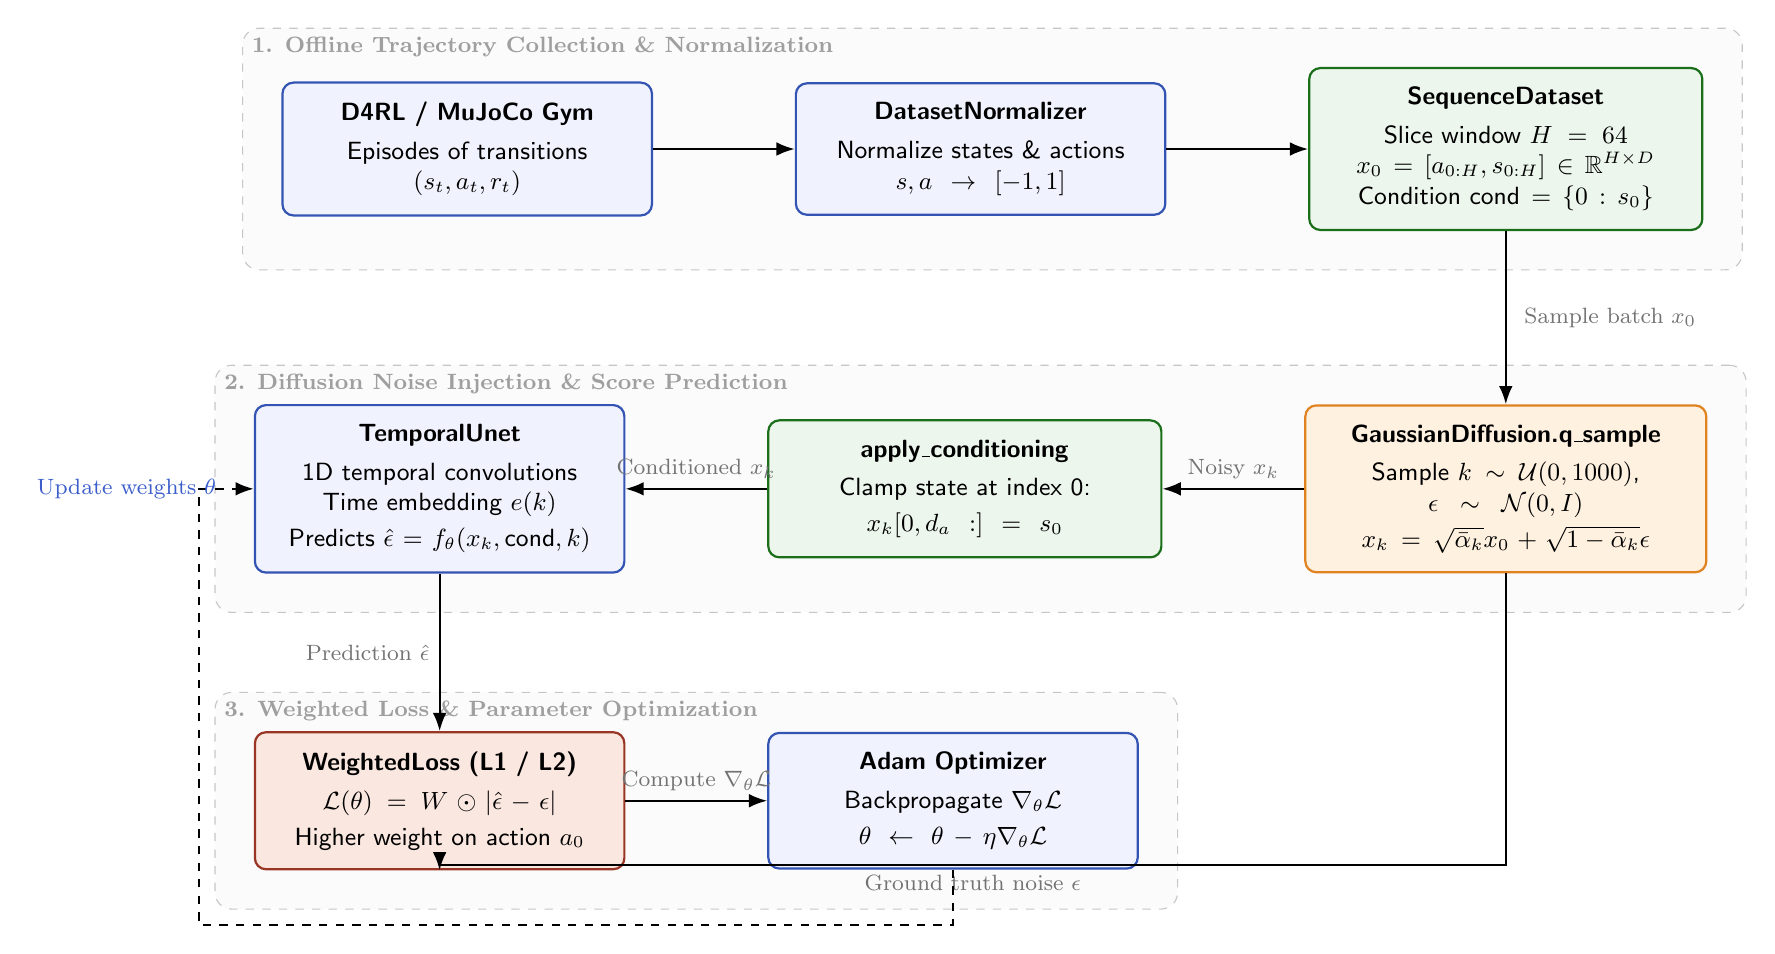
\begin{tikzpicture}[
    >=Latex,
    font=\sffamily\small,
    node distance=1.6cm and 1.8cm,
    block/.style={
        rectangle, 
        draw=RoyalBlue!80!black, 
        fill=RoyalBlue!8, 
        rounded corners=4pt, 
        align=center,
        text width=4.2cm, 
        minimum height=1.4cm, 
        inner sep=7pt,
        line width=0.8pt
    },
    data/.style={
        rectangle, 
        draw=ForestGreen!80!black, 
        fill=ForestGreen!8, 
        rounded corners=4pt, 
        align=center,
        text width=4.5cm, 
        minimum height=1.4cm, 
        inner sep=7pt,
        line width=0.8pt
    },
    op/.style={
        rectangle, 
        draw=BurntOrange!90!black, 
        fill=BurntOrange!10, 
        rounded corners=4pt, 
        align=center,
        text width=4.6cm, 
        minimum height=1.4cm, 
        inner sep=7pt,
        line width=0.8pt
    },
    loss/.style={
        rectangle, 
        draw=BrickRed!80!black, 
        fill=BrickRed!8, 
        rounded corners=4pt, 
        align=center,
        text width=4.2cm, 
        minimum height=1.4cm, 
        inner sep=7pt,
        line width=0.8pt
    },
    groupbox/.style={
        draw=gray!45, 
        dashed, 
        rounded corners=6pt, 
        inner sep=14pt, 
        fill=gray!3
    }
]

% Row 1: Offline Trajectory Collection & Formatting
\node[block] (env) {\textbf{D4RL / MuJoCo Gym}\\[3pt]Episodes of transitions\\$(s_t, a_t, r_t)$};

\node[block, right=of env] (norm) {\textbf{DatasetNormalizer}\\[3pt]Normalize states \& actions\\$s, a \to [-1, 1]$};

\node[data, right=of norm] (seq) {\textbf{SequenceDataset}\\[3pt]Slice window $H=64$\\$x_0 = [a_{0:H}, s_{0:H}] \in \mathbb{R}^{H \times D}$\\Condition $\text{cond} = \{0: s_0\}$};

% Row 2: Forward Diffusion & Score Modeling
\node[op, below=2.2cm of seq] (noise) {\textbf{GaussianDiffusion.q\_sample}\\[3pt]Sample $k \sim \mathcal{U}(0, 1000)$, $\epsilon \sim \mathcal{N}(0, I)$\\[2pt]$x_k = \sqrt{\bar{\alpha}_k} x_0 + \sqrt{1 - \bar{\alpha}_k}\epsilon$};

\node[data, left=of noise] (cond) {\textbf{apply\_conditioning}\\[3pt]Clamp state at index 0:\\[2pt]$x_k[0, d_a:] = s_0$};

\node[block, left=of cond] (unet) {\textbf{TemporalUnet}\\[3pt]1D temporal convolutions\\Time embedding $e(k)$\\[2pt]Predicts $\hat{\epsilon} = f_\theta(x_k, \text{cond}, k)$};

% Row 3: Loss Computation & Parameter Updates
\node[loss, below=2.0cm of unet] (lossnode) {\textbf{WeightedLoss (L1 / L2)}\\[3pt]$\mathcal{L}(\theta) = W \odot |\hat{\epsilon} - \epsilon|$\\[2pt]Higher weight on action $a_0$};

\node[block, right=of lossnode] (opt) {\textbf{Adam Optimizer}\\[3pt]Backpropagate $\nabla_\theta \mathcal{L}$\\[2pt]$\theta \leftarrow \theta - \eta \nabla_\theta \mathcal{L}$};

% Connectors Row 1
\draw[->, thick] (env) -- (norm);
\draw[->, thick] (norm) -- (seq);

% Row 1 to Row 2
\draw[->, thick] (seq) -- node[right, font=\footnotesize, text=gray!90!black, xshift=3pt] {Sample batch $x_0$} (noise);

% Connectors Row 2
\draw[->, thick] (noise) -- node[above, font=\footnotesize, text=gray!90!black] {Noisy $x_k$} (cond);
\draw[->, thick] (cond) -- node[above, font=\footnotesize, text=gray!90!black] {Conditioned $x_k$} (unet);

% Row 2 to Row 3
\draw[->, thick] (unet.south) -- node[left, font=\footnotesize, text=gray!90!black] {Prediction $\hat{\epsilon}$} (lossnode.north);

% Target noise to lossnode routed cleanly underneath row 3
\draw[->, thick] (noise.south) -- ++(0,-3.7) -| node[pos=0.25, below, font=\footnotesize, text=gray!90!black] {Ground truth noise $\epsilon$} (lossnode.south);

% Connectors Row 3
\draw[->, thick] (lossnode) -- node[above, font=\footnotesize, text=gray!90!black] {Compute $\nabla_\theta \mathcal{L}$} (opt);

% Parameter update routed cleanly around the left
\draw[->, thick, dashed] (opt.south) -- ++(0,-0.7) -| ([xshift=-0.7cm]lossnode.west) |- node[pos=0.75, left, font=\footnotesize, text=RoyalBlue!90!black] {Update weights $\theta$} (unet.west);

% Group backgrounds
\begin{scope}[on background layer]
    \node[groupbox, fit=(env)(norm)(seq), label={[anchor=north west, font=\bfseries\footnotesize, text=gray!75]north west:1. Offline Trajectory Collection \& Normalization}] (g1) {};
    \node[groupbox, fit=(noise)(cond)(unet), label={[anchor=north west, font=\bfseries\footnotesize, text=gray!75]north west:2. Diffusion Noise Injection \& Score Prediction}] (g2) {};
    \node[groupbox, fit=(lossnode)(opt), label={[anchor=north west, font=\bfseries\footnotesize, text=gray!75]north west:3. Weighted Loss \& Parameter Optimization}] (g3) {};
\end{scope}

\end{tikzpicture}
\end{document}
